
\begin{frame}{pointer authentication use}
    \begin{itemize}
    \item commonly enabled on ARM64 for return addreses
    \vspace{.25cm}
    \item otherwise:
    \item on ARM64 OS X --- used by OS X
        \begin{itemize}
        \item two different compiler `architectures': arm64, arm64e
        \item can't use arm64e libraries in arm64 program or vice-versa
        \end{itemize}
    \item proposals to use on Linux in global offset table, etc.
        \begin{itemize}
        \item GNU Linux linker option -z pac-plt; unclear if used `for real'
        \end{itemize}
    \end{itemize}
\end{frame}

\begin{frame}[fragile]{macOS PAC for apple code}
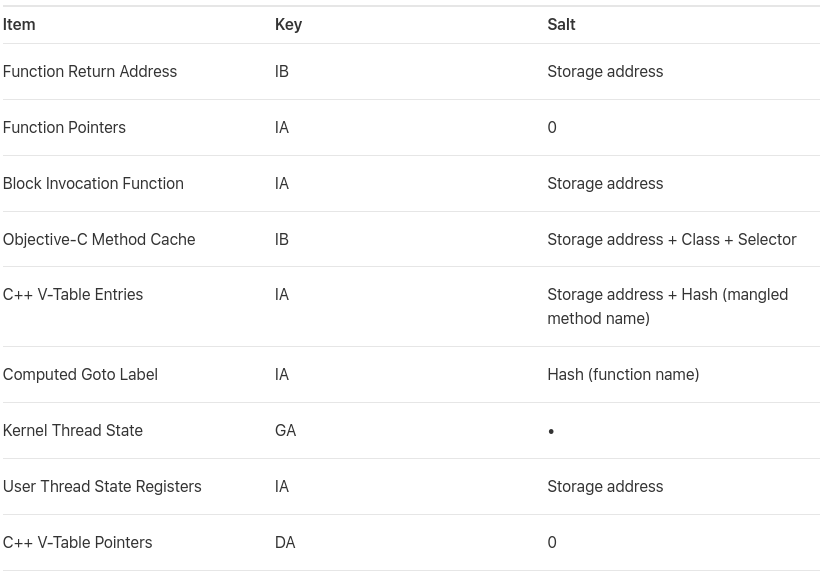
\includegraphics[height=0.9\textheight]{../cfi/apple-pac-usage}
\imagecredit{\url{https://support.apple.com/en-il/guide/security/sec8b776536b/1/web/1}}
\end{frame}

\begin{frame}{macOS PAC}
    \begin{itemize}
    \item `new' `preview' architecture in compiter
    \item seems to be used internally by Apple
    \item doesn't appear easily available/supported for others
    \item incompatible with `old' libraries
    \end{itemize}
\end{frame}

\begin{frame}{PAC bypasses}
    \begin{itemize}
    \item have been exploits in spite of PAC in iOS kernel
    \vspace{.5cm}
    \item only certain code pointers authenticated
        \begin{itemize}
        \item too expensive to authenticate all pointers
        \end{itemize}
    \item changing unsigned pointer values just before signed 
        \begin{itemize}
        \item get context switch to occur at just the right time
        \item modify pointer value in saved context
        \end{itemize}
    \item code that signs pointers they shouldn't
        \begin{itemize}
        \item changing pointer without crashing if old pointer invalid
        \end{itemize}
    \item `gadgets' that allow brute-forcing MAC tag
        \begin{itemize}
        \item not enough space in pointers for non-brute-forceable tag
        \end{itemize}
    \end{itemize}
\end{frame}
